% Technical report: place in ~/lidar_loop/docs/report/report.tex and compile with
%   pdflatex report.tex && pdflatex report.tex
% Figures are read from ../figures/ (docs/figures/traj_seq05.pdf, traj_seq08.pdf).
\documentclass[11pt,a4paper]{article}
\usepackage[margin=2.3cm]{geometry}
\usepackage{amsmath,amssymb}
\usepackage{graphicx}
\usepackage{booktabs}
\usepackage{caption}
\usepackage{subcaption}
\usepackage[hidelinks]{hyperref}
\graphicspath{{../figures/}}

\title{When Accurate Loop Closures Hurt Local Accuracy:\\
Diagnosing and Fixing Factor Weighting in KISS-SLAM on KITTI}
\author{Yassine Mtibaa\\
South Mediterranean University (MedTech), Tunis, Tunisia\\
\texttt{yassine.mtibaa@medtech.tn}}
\date{Technical report, October 2026}

\begin{document}
\maketitle

\begin{abstract}
Loop closure is expected to improve a SLAM trajectory. Evaluating the open-source LiDAR SLAM system KISS-SLAM
on the KITTI odometry benchmark, we find that it reduces global error (ATE) by up to 74\% but increases local
error, measured by the KITTI translation metric, by up to 51\% relative to its own odometry. An audit shows that
all accepted closures on the tuning sequences are more accurate than the odometry they replace, so the loss does
not come from wrong closures. Disabling closures removes 86--96\% of the loss, and the corrections the
optimizer applies are uncorrelated with where the odometry actually drifted. The code assigns an identity
information matrix to every pose-graph factor, which weights one radian of rotation like one metre of
translation and makes heading changes nearly free. Weighting the rotational block $10^3$ times more
heavily, a two-line change, brings the local error of the most affected tuning sequence from 0.517\% to
0.333\% (odometry: 0.342\%) while reducing its ATE from 0.66\,m to 0.36\,m. On the held-out test sequence~08,
where default loop closure made the trajectory worse than odometry, the change reduces local error from
0.954\% to 0.841\% and ATE from 2.52\,m to 2.13\,m (odometry: 2.27\,m). All hypotheses and acceptance rules were
written down before each run; failed predictions are reported. A secondary finding characterizes a
structured range artifact in the Gazebo \texttt{gpu\_lidar} sensor that exceeds real LiDAR noise beyond about
8\,m.
\end{abstract}

\section{Introduction}
Pose-graph SLAM corrects accumulated odometry drift by adding loop-closure constraints and re-optimizing the
graph. Global consistency usually improves, but the way the correction is distributed along the trajectory
depends on how the factors are weighted. Learning-based systems such as MAC-VO~\cite{macvo} show that
metrics-aware covariances in the pose graph improve visual odometry; many LiDAR pipelines, however, still use
fixed or identity weights.

This report studies KISS-SLAM~\cite{kissslam}, which combines KISS-ICP odometry~\cite{kissicp} with
density-map loop closures and pose-graph optimization. The contributions are:
\begin{enumerate}
  \item a measurement showing that default loop closure trades local accuracy for global accuracy on several
        KITTI sequences, even when every closure is accurate;
  \item a step-by-step diagnosis that rules out closure errors, the odometry front-end, and the optimizer's
        iteration limit, and points to identity factor weighting;
  \item a two-line fix (rotation-weighted information matrices) evaluated with a tuning/validation/test split,
        including a held-out sequence on which it turns a net loss into a net gain;
  \item a characterization of a range artifact in the Gazebo GPU LiDAR simulator, relevant to anyone using it
        for noise modelling.
\end{enumerate}

\section{Setup and methodology}
\paragraph{Data and software.} KITTI odometry~\cite{kitti} sequences 00--10 (Velodyne HDL-64E, ground truth
available). KISS-ICP~1.3.0 and KISS-SLAM~0.0.2 installed via \texttt{pipx}; evaluation with
\texttt{evo}~1.37.1~\cite{evo}; Ubuntu~24.04, RTX~4060 laptop GPU, 32\,GB RAM. KISS-SLAM's pose graph is
solved with a g2o-based optimizer~\cite{g2o}.

\paragraph{Metrics.} ATE: RMSE of absolute position error after SE(3) alignment (\texttt{evo\_ape -a}).
RPE: RMSE of translational error over 100\,m segments (\texttt{evo\_rpe -d 100}). KITTI translation error:
the benchmark's average over 100--800\,m segments, in percent. ATE measures global consistency; RPE and the
KITTI metric measure local accuracy.

\paragraph{Split and discipline.} Sequences 00--05 were used for tuning, 06--07 for validation, and 08--10
for a single final test. Before every experiment, the hypothesis, the predicted outcome and the acceptance
rule were committed to a decision log; results were then recorded whether or not they confirmed the
prediction. KISS-ICP was verified to be deterministic (a parallel rerun reproduced all metrics exactly).
KISS-SLAM is deterministic on 05, 06, 07 and 08--10, but on 02 the number of accepted closures flips between
1 and 2 across runs (ATE spread 3.3\%), and 00 shows a 1.1\% ATE spread; differences below these bands are
treated as noise.

\section{Baselines}
A sweep of KISS-ICP preprocessing parameters (deskewing, minimum and maximum range, voxel size) found no
configuration that improved mean RPE on the tuning sequences by the pre-set 2\% margin; the defaults are close
to optimal on KITTI. Table~\ref{tab:base} compares KISS-ICP odometry with default KISS-SLAM.

\begin{table}[h]
\centering
\small
\begin{tabular}{lrrrrrr}
\toprule
 & \multicolumn{2}{c}{ATE (m)} & \multicolumn{2}{c}{KITTI trans.\ error (\%)} & & \\
\cmidrule(lr){2-3}\cmidrule(lr){4-5}
Seq. & Odometry & SLAM & Odometry & SLAM & Change & Closures \\
\midrule
00 & 3.501 & 0.907 & 0.528 & 0.573 & +8.5\% & 7 \\
01 & 3.149 & 3.117 & 0.786 & 0.798 & +1.5\% & 0 \\
02 & 6.463 & 1.854 & 0.537 & 0.580 & +8.0\% & 2 \\
03 & 0.515 & 0.528 & 0.677 & 0.674 & $-$0.4\% & 0 \\
04 & 0.241 & 0.243 & 0.385 & 0.384 & $-$0.3\% & 0 \\
05 & 1.491 & 0.661 & 0.342 & 0.517 & +51\% & 5 \\
06 & 0.418 & 0.328 & 0.281 & 0.325 & +16\% & 4 \\
07 & 0.315 & 0.315 & 0.375 & 0.386 & +2.9\% & 1 \\
08 & 2.266 & 2.524 & 0.820 & 0.954 & +16\% & 5 \\
09 & 1.308 & 1.259 & 0.534 & 0.542 & +1.5\% & 0 \\
10 & 0.709 & 0.718 & 0.512 & 0.525 & +2.5\% & 0 \\
\bottomrule
\end{tabular}
\caption{KISS-ICP odometry versus default KISS-SLAM. Loop closure reduces ATE by 56--74\% on 00, 02 and 05,
but increases local error on every sequence with several closures. On 08 it also worsens ATE.}
\label{tab:base}
\end{table}

\section{Diagnosis}
Each step below tested one explanation for the local-accuracy loss, with the prediction fixed in advance.

\paragraph{Are the closures wrong?} No. For each of the 14 closures accepted on 00, 02 and 05, the relative pose
was compared with ground truth and with the relative pose implied by odometry between the same scans. Every
closure was more accurate than the odometry chain it replaces (closure errors 0.12--4.88\,m against
0.91--18.1\,m), and the overlap score used for acceptance did not visibly predict closure error.

\paragraph{Is it the odometry inside KISS-SLAM?} No. With closures disabled (overlap threshold 1.0), KISS-SLAM
matches standalone odometry: KITTI error 0.349\% on 05 (odometry 0.342\%, default 0.517\%), 0.532\% on 00 and
0.543\% on 02. Between 86\% and 96\% of the gap appears only when closures are applied.

\paragraph{Is the optimizer stopping early?} No. Raising the iteration limit from 10 to 50 or 100 left 05
unchanged to six digits.

\paragraph{Where do the corrections go?} For each 100\,m segment we compared the change introduced by the
optimizer with the segment's odometry error. The correlation between correction size and odometry error was
0.13 (05), $-$0.11 (00) and 0.23 (02); on 05 the root-mean-square correction per segment (0.49\,m) was about
seven times larger than the evenly distributed drift (about 0.07\,m). Removing three of the five closures on
05 shrank the corrections in the affected span by 91\% and restored odometry-level local accuracy, but the
same intervention had no effect on 00 and 02, so closure selection alone is not a general explanation.

\paragraph{Mechanism.} In the KISS-SLAM source, every factor (between local maps, loop closures, and the final
per-scan refinement) is added with \texttt{np.eye(6)}. Odometry over 100\,m drifts on the order of 0.5\,m in
translation but only about 0.1$^\circ$ (0.0017\,rad) in heading, so a physically consistent weighting would make
rotation roughly $(0.5/0.0017)^2 \approx 10^5$ times more expensive than an identity matrix does. With identity
weights, the optimizer can satisfy a closure by bending headings almost for free, distributing the correction
where the odometry was in fact accurate.

\section{Fix and evaluation}
The patch reads the diagonal of each information matrix from an environment variable and falls back to
\texttt{np.eye(6)} when unset (verified to reproduce the default exactly on 05). The rotational block is
weighted by $W$: $\Lambda=\mathrm{diag}(1,1,1,W,W,W)$, applied to all factors.

\paragraph{Round 1 (00, 02, 05).} Weighting the last three entries by $10^4$ reduced 05's KITTI error to
0.341\%; weighting the first three by $10^4$ instead increased it to 0.725\%, which identifies the last block as
rotation. The prediction that only one of the two variants would matter was wrong: only the ratio between the
blocks matters, so the second variant made rotation cheaper still. Uniformly down-weighting closures by 10
also helped 05 (0.392\%) but raised 02's ATE by 17\%, outside its noise band.

\paragraph{Weight selection (00--05).} The selection rule, fixed in advance, picked the $W\in\{10^3,10^4,10^5\}$
with the largest mean improvement in KITTI error, subject to no sequence losing more than 20\% ATE or 5\% KITTI
error. Mean changes were $-5.5\%$, $-4.7\%$ and $-4.7\%$; $W=10^3$ was selected. Loop-free sequences 01, 03 and
04 were unchanged. On 05, $W=10^3$ gives 0.333\% (odometry 0.342\%) and ATE 0.364\,m (default 0.661\,m); the cost
on 00 is +1.9\%. The gain was already saturated at the smallest weight tested, so the optimum may lie lower;
this was not explored to avoid post-hoc tuning.

\paragraph{Validation and test.} Table~\ref{tab:test} reports the single runs on validation and test sequences.
Both validation sequences pass the pre-set rule. On the held-out sequence 08, default loop closure made the
trajectory worse than odometry in both metrics; with $W=10^3$ it becomes better than odometry in ATE and loses
only 2.6\% in local accuracy. Sequences 09 and 10 have no accepted closures and are unchanged. Repeated default
runs on 08--10 were identical, so the 08 difference is not run-to-run noise.

\begin{table}[h]
\centering
\small
\begin{tabular}{llrrrrrr}
\toprule
 & & \multicolumn{3}{c}{KITTI trans.\ error (\%)} & \multicolumn{3}{c}{ATE (m)} \\
\cmidrule(lr){3-5}\cmidrule(lr){6-8}
Role & Seq. & Odometry & Default & $W=10^3$ & Odometry & Default & $W=10^3$ \\
\midrule
Validation & 06 & 0.281 & 0.325 & 0.332 & 0.418 & 0.328 & 0.331 \\
Validation & 07 & 0.375 & 0.386 & 0.391 & 0.314 & 0.315 & 0.314 \\
Test & 08 & 0.820 & 0.954 & \textbf{0.841} & 2.266 & 2.524 & \textbf{2.126} \\
Test & 09 & 0.534 & 0.542 & 0.542 & 1.309 & 1.259 & 1.256 \\
Test & 10 & 0.512 & 0.525 & 0.525 & 0.710 & 0.718 & 0.718 \\
\bottomrule
\end{tabular}
\caption{Validation and test results, each run once after $W$ was fixed on the tuning sequences.}
\label{tab:test}
\end{table}

\begin{figure}[h]
\centering
\begin{subfigure}{0.49\linewidth}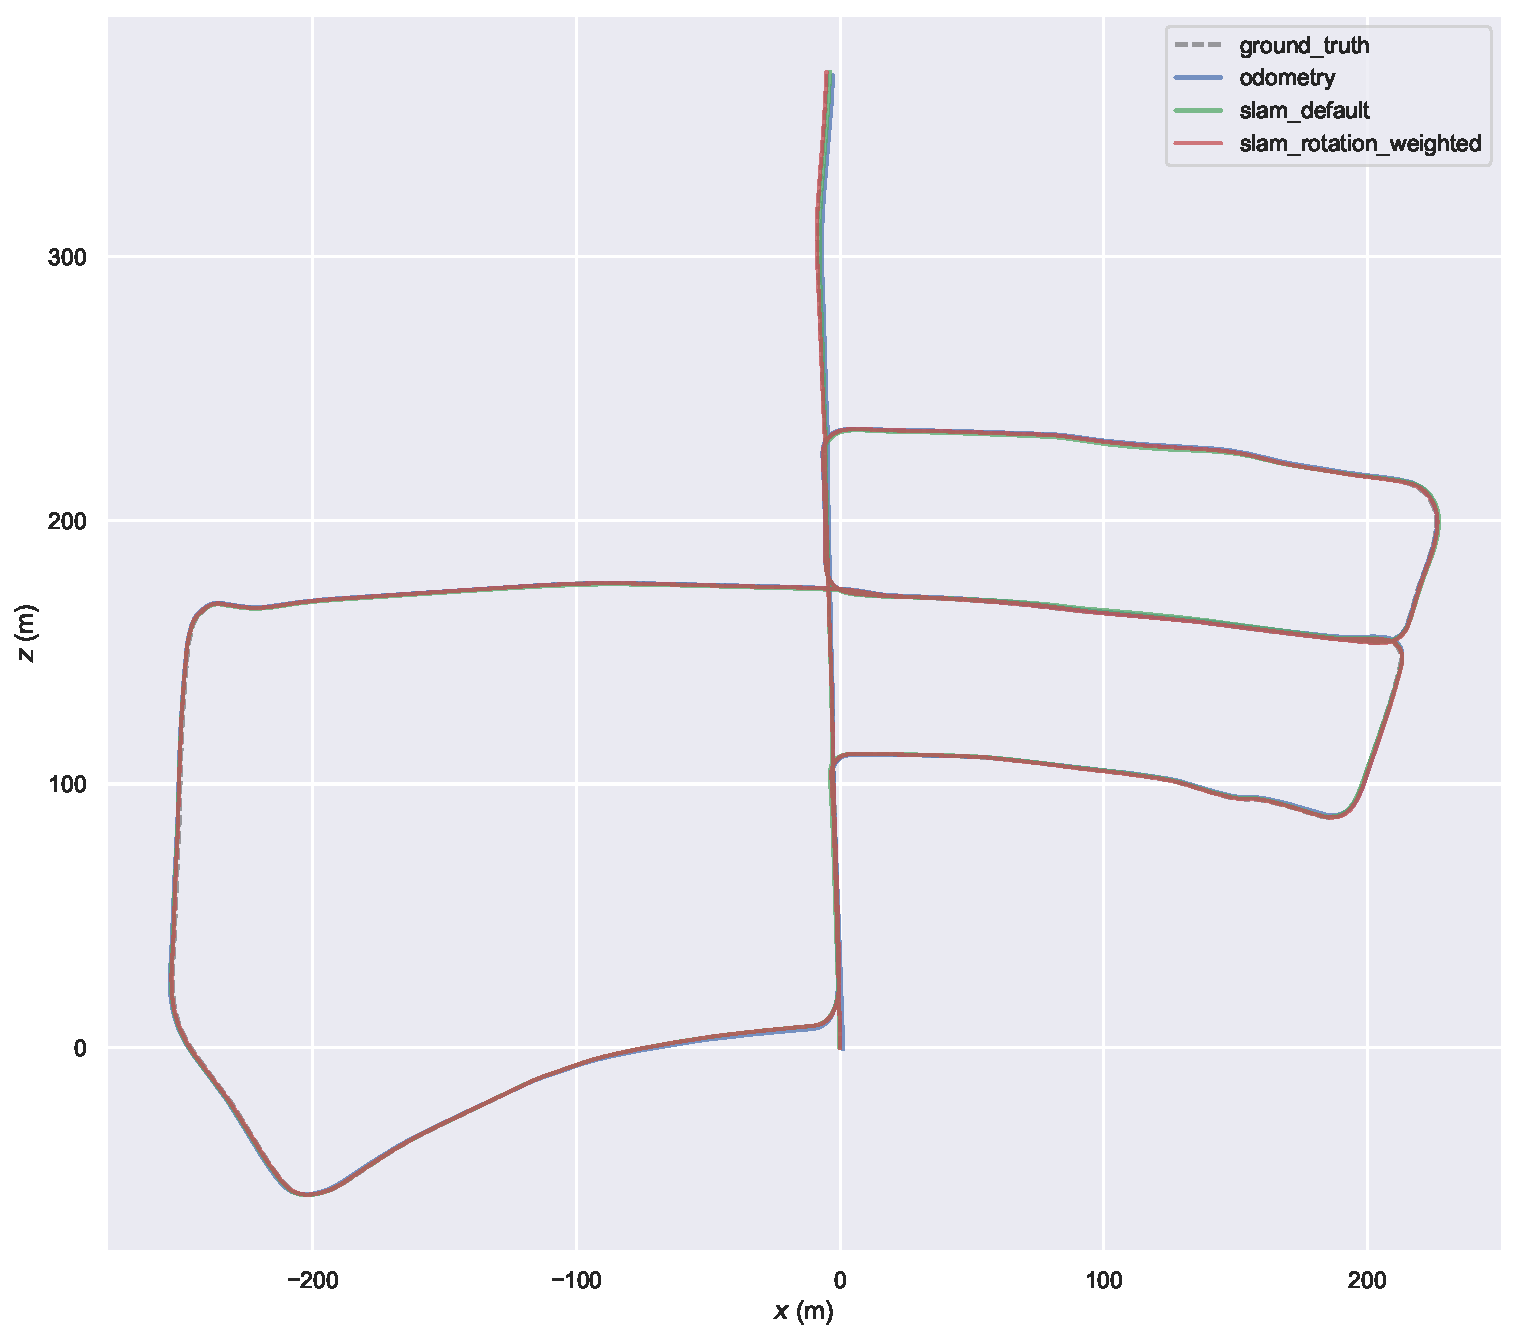
\includegraphics[width=\linewidth]{traj_seq05.pdf}\caption{Sequence 05 (tuning)}\end{subfigure}
\begin{subfigure}{0.49\linewidth}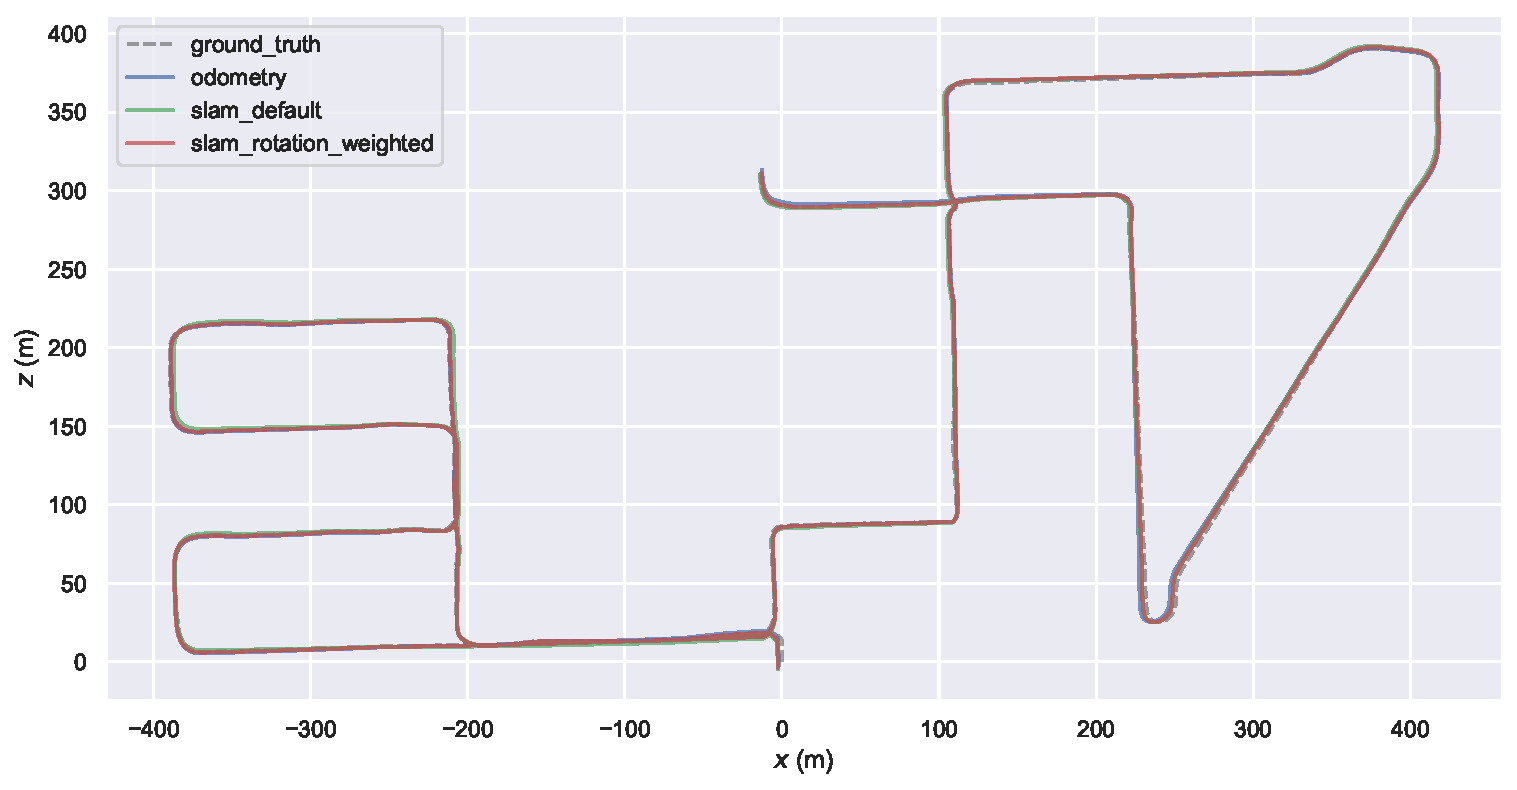
\includegraphics[width=\linewidth]{traj_seq08.pdf}\caption{Sequence 08 (test)}\end{subfigure}
\caption{Top-down trajectories (x--z plane): ground truth, KISS-ICP odometry, default KISS-SLAM and
rotation-weighted KISS-SLAM ($W=10^3$), aligned to ground truth.}
\end{figure}

\section{Secondary finding: a range artifact in Gazebo's GPU LiDAR}
To model sensor noise for simulation, range noise was measured on KITTI by second differences along each
beam on road surface, an estimator verified to within 1\% on synthetic white noise. It gives 0.84--0.90\,cm at
3--10\,m and 1.65--1.83\,cm at 30--40\,m (sequences 00, 02, 05), an upper bound on white range noise. Plane-fit
residuals, by contrast, are 4--8\,cm and measure road shape rather than the sensor.

In Gazebo Sim~8 (Harmonic), a 64-beam \texttt{gpu\_lidar} over a flat ground plane showed two artifacts. A
360$^\circ$ configuration returned spurious points 1--1.6\,m from the sensor over most azimuths; a 120$^\circ$
sector did not. Within the clean sector, the ideal (noise-free) ranges contain deterministic jumps: about 40\% of
ground triples include a step, 88\% of steps appear as adjacent opposite-sign pairs, and the step size is about
0.19\% of range beyond 8\,m. Changing the sensor's minimum range had no effect. The resulting second-difference
spread (2.6\,cm at 9\,m, 15\,cm at 29\,m) exceeds the real sensor noise beyond about 8\,m, by roughly ten times
at 30\,m, so adding a realistic noise model on top of this sensor does not produce realistic data at range. The
cause of the jumps was not identified. A noise-injection ROS~2 node was implemented and verified (injected and
measured noise agree within 2\%).

\section{Limitations}
All results come from one dataset, one SLAM system and one sensor. The effect is large on two sequences (05 and
08) and small or absent elsewhere; the local loss on 06 is not recovered. $W$ was chosen from three candidates and
the information matrix is a scaled identity, not a calibrated covariance. KISS-SLAM is not fully deterministic on
some sequences. The simulator findings concern one Gazebo version and a flat-ground statistic.

\section{Conclusion and future work}
Identity information matrices let a pose-graph optimizer absorb loop-closure corrections as cheap heading changes,
which costs local accuracy even when every closure is accurate. Weighting rotation consistently with the physical
scale of odometry error removes most of that cost on the affected KITTI sequences, including a held-out one,
while improving global consistency. Natural next steps are per-factor covariances estimated from the registration
itself, evaluation on datasets with more loops and more degenerate scenes~\cite{superloc}, and learned covariances
where the classical estimates fail.

\paragraph{Reproducibility.} Code, configurations, the decision log with every prediction and result, and the
patch are available at \url{https://github.com/yassinmtibaa/lidar-loop-closure-weighting}.

\begin{thebibliography}{9}
\bibitem{kitti} A.~Geiger, P.~Lenz, R.~Urtasun. Are we ready for autonomous driving? The KITTI vision benchmark
suite. \emph{CVPR}, 2012.
\bibitem{kissicp} I.~Vizzo, T.~Guadagnino, B.~Mersch, L.~Wiesmann, J.~Behley, C.~Stachniss. KISS-ICP: In defense of
point-to-point ICP -- simple, accurate, and robust registration if done the right way. \emph{IEEE Robotics and
Automation Letters}, 2023; arXiv:2209.15397.
\bibitem{kissslam} T.~Guadagnino, B.~Mersch, S.~Gupta, I.~Vizzo, G.~Grisetti, C.~Stachniss. KISS-SLAM: a simple,
robust, and accurate 3D LiDAR SLAM system with enhanced generalization capabilities. \emph{IROS}, 2025;
arXiv:2503.12660.
\bibitem{g2o} R.~K\"ummerle, G.~Grisetti, H.~Strasdat, K.~Konolige, W.~Burgard. g2o: A general framework for graph
optimization. \emph{ICRA}, 2011.
\bibitem{evo} M.~Grupp. evo: Python package for the evaluation of odometry and SLAM.
\url{https://github.com/MichaelGrupp/evo}, 2017.
\bibitem{macvo} Y.~Qiu, Y.~Chen, Z.~Zhang, W.~Wang, S.~Scherer. MAC-VO: Metrics-aware covariance for learning-based
stereo visual odometry. arXiv:2409.09479, 2024.
\bibitem{superloc} S.~Zhao, H.~Zhu, Y.~Gao, B.~Kim, Y.~Qiu, A.~M.~Johnson, S.~Scherer. SuperLoc: The key to robust
LiDAR-inertial localization lies in predicting alignment risks. arXiv:2412.02901, 2024.
\end{thebibliography}

\end{document}
